\sectionframe{Recap}
\section{Recap}

\begin{frame}{Definition of Minimal Reproducing Model (1/2)}
    \vspace{-3.0em}
    \begin{align}
        x \mapsto f(x) \mod 1
    \end{align}

    \begin{align}
        f(x) & = \begin{cases}
                     g(x)                                        & \text{ if } x < \frac{1}{2} \\
                     g\left(x - \frac{1}{2}\right) + \frac{1}{2} & \text{ else}
                 \end{cases}
    \end{align}

    \begin{align}
        g(x) & = \begin{cases}
                     l(x) = a_L \cdot x^2 + b_L \cdot x + c_L & \text{ if } x < \frac{1}{4} \\
                     r(x) = b_R \cdot x + c_R                 & \text{ else}
                 \end{cases}
    \end{align}
\end{frame}

\begin{frame}{Definition of Minimal Reproducing Model (2/2)}
    \vspace{-1em}
    \begin{columns}
        \begin{column}{.7 \textwidth}
            Fixed parameters:
            \begin{align*}
                a_L = 4, b_L = -\frac{1}{2}
            \end{align*}

            Variable parameters
            \begin{align*}
                 & c_L, b_R, c_R                                                    \\
                \text{where} \qquad
                 & c_L = p_y,                                                       \\
                 & b_R = 4 \cdot (B - A), c_R = 2A - B                              \\
                \text {and} \qquad
                 & A = p_x, \text{and } B = \frac{1}{2} + \epsilon \text{ is fixed}
            \end{align*}

            $A$ and $B$ are intermediated parameters for modeling the values of the left ($A$) and right ($B$) borders of $r(x)$
        \end{column}
        \begin{column}{.3 \textwidth}
            \begin{figure}
                \centering
                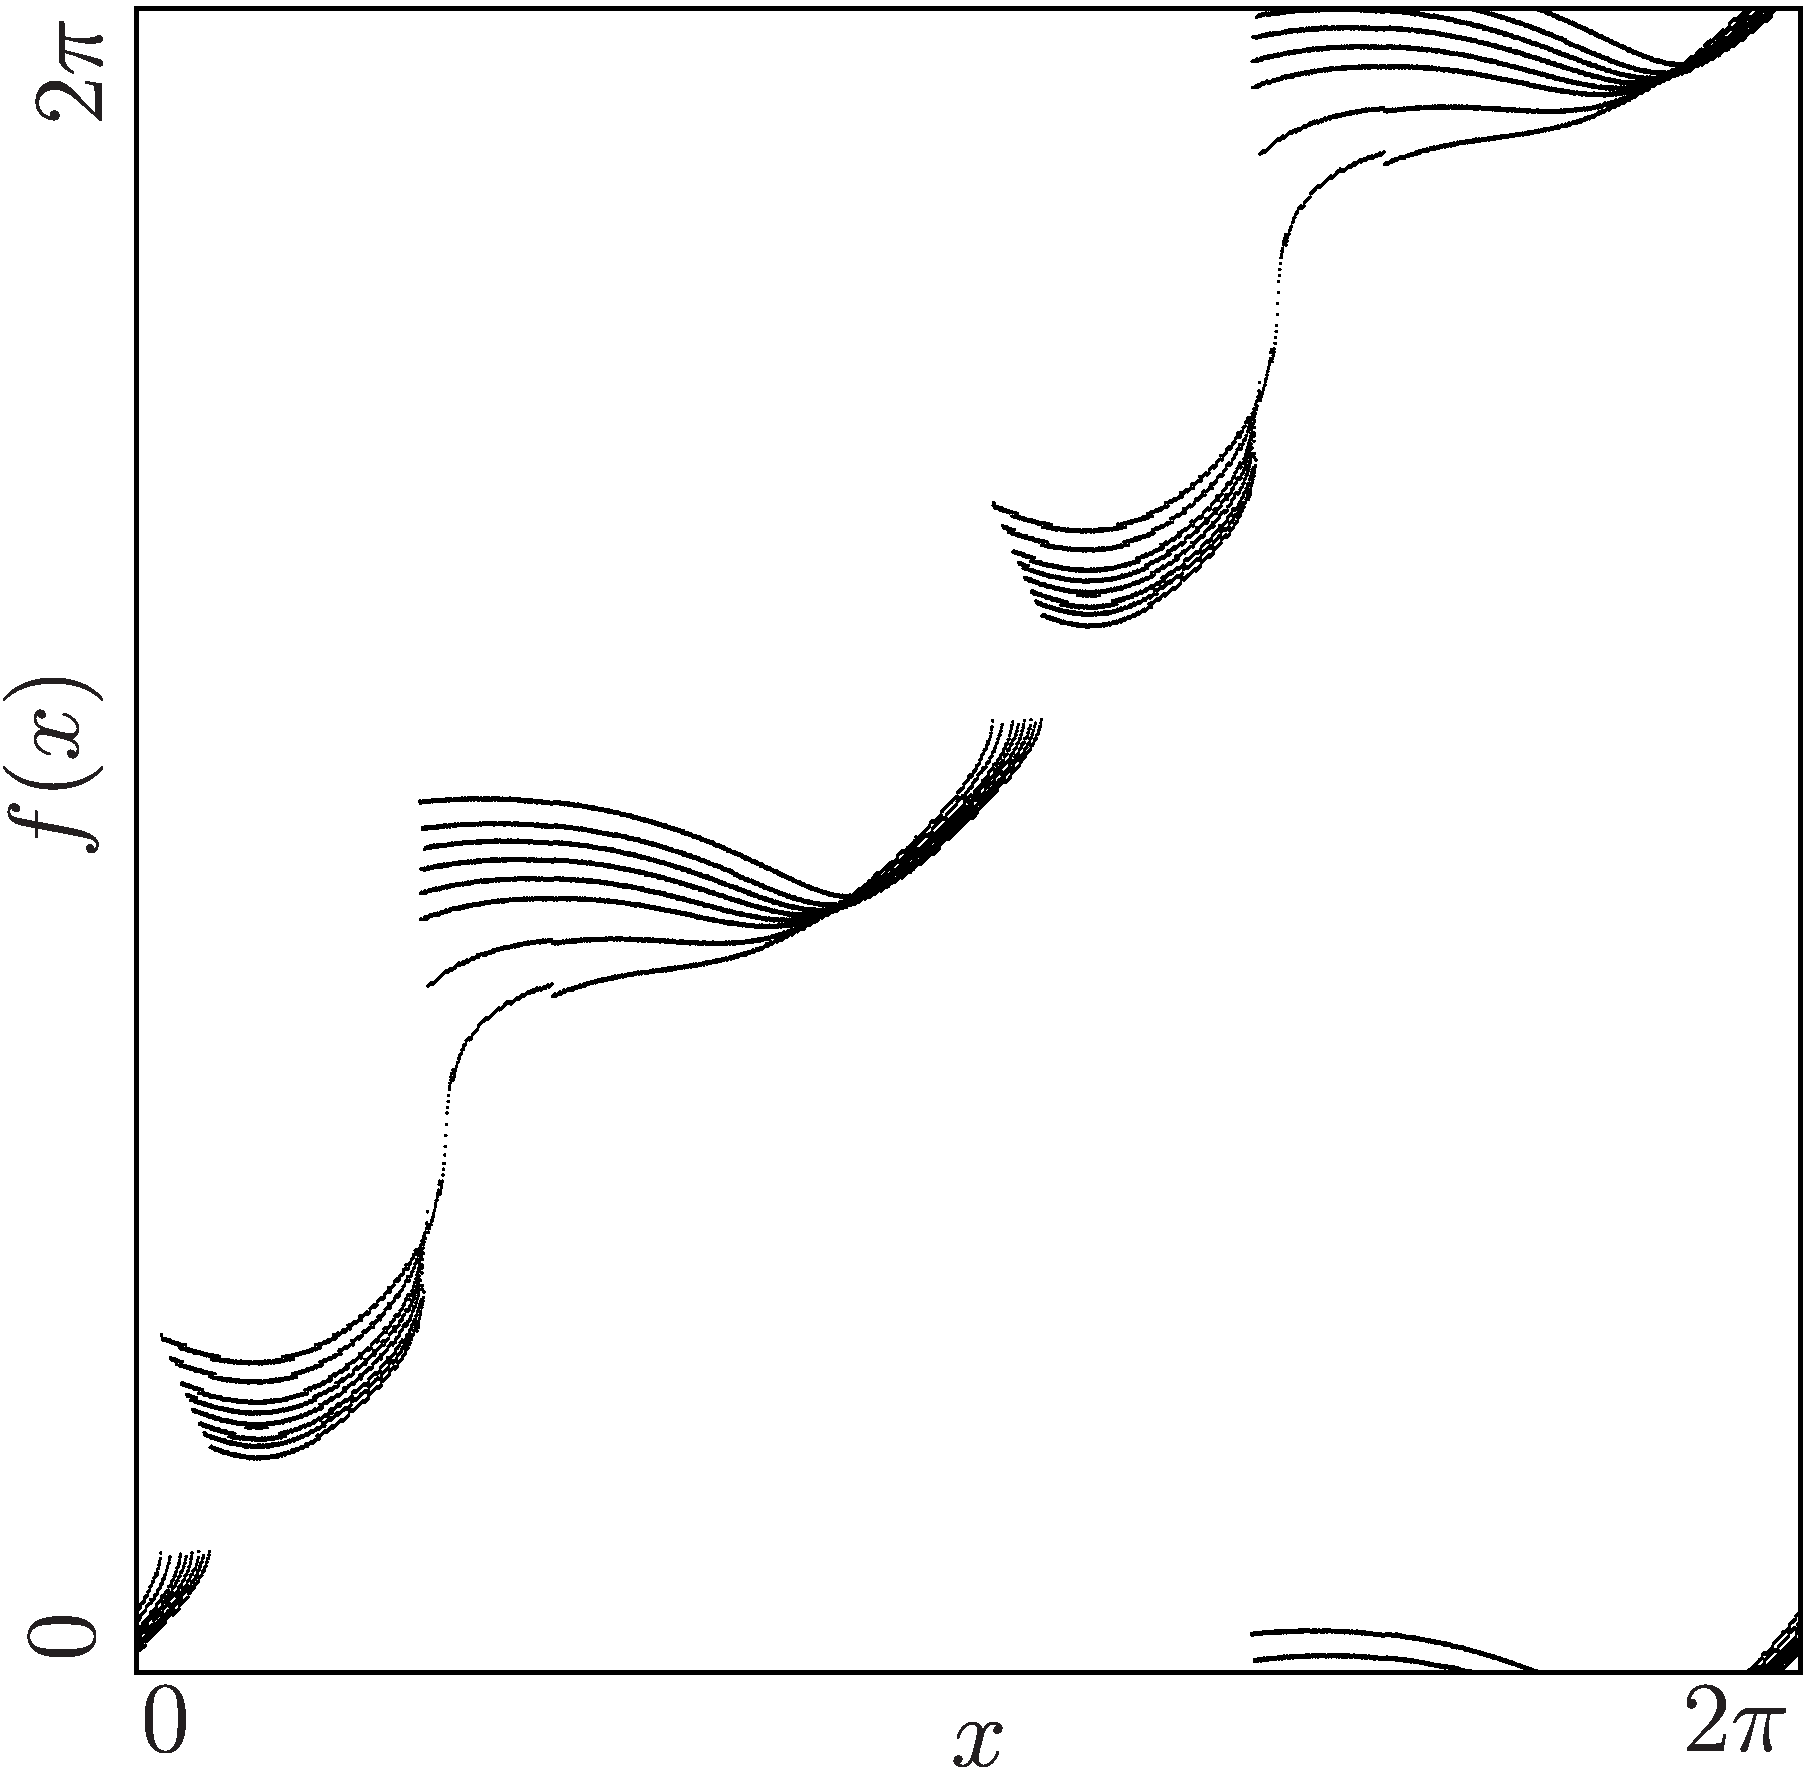
\includegraphics[height=.5 \textheight]{60_MinimalRepr/ParameterEffects/AB/illustration.png}
                \caption*{Illustration of the parameters $A$ and $B$}
            \end{figure}
        \end{column}
    \end{columns}
\end{frame}

\begin{frame}{Minimal Reproducing Model Dynamics}
    \begin{center}
        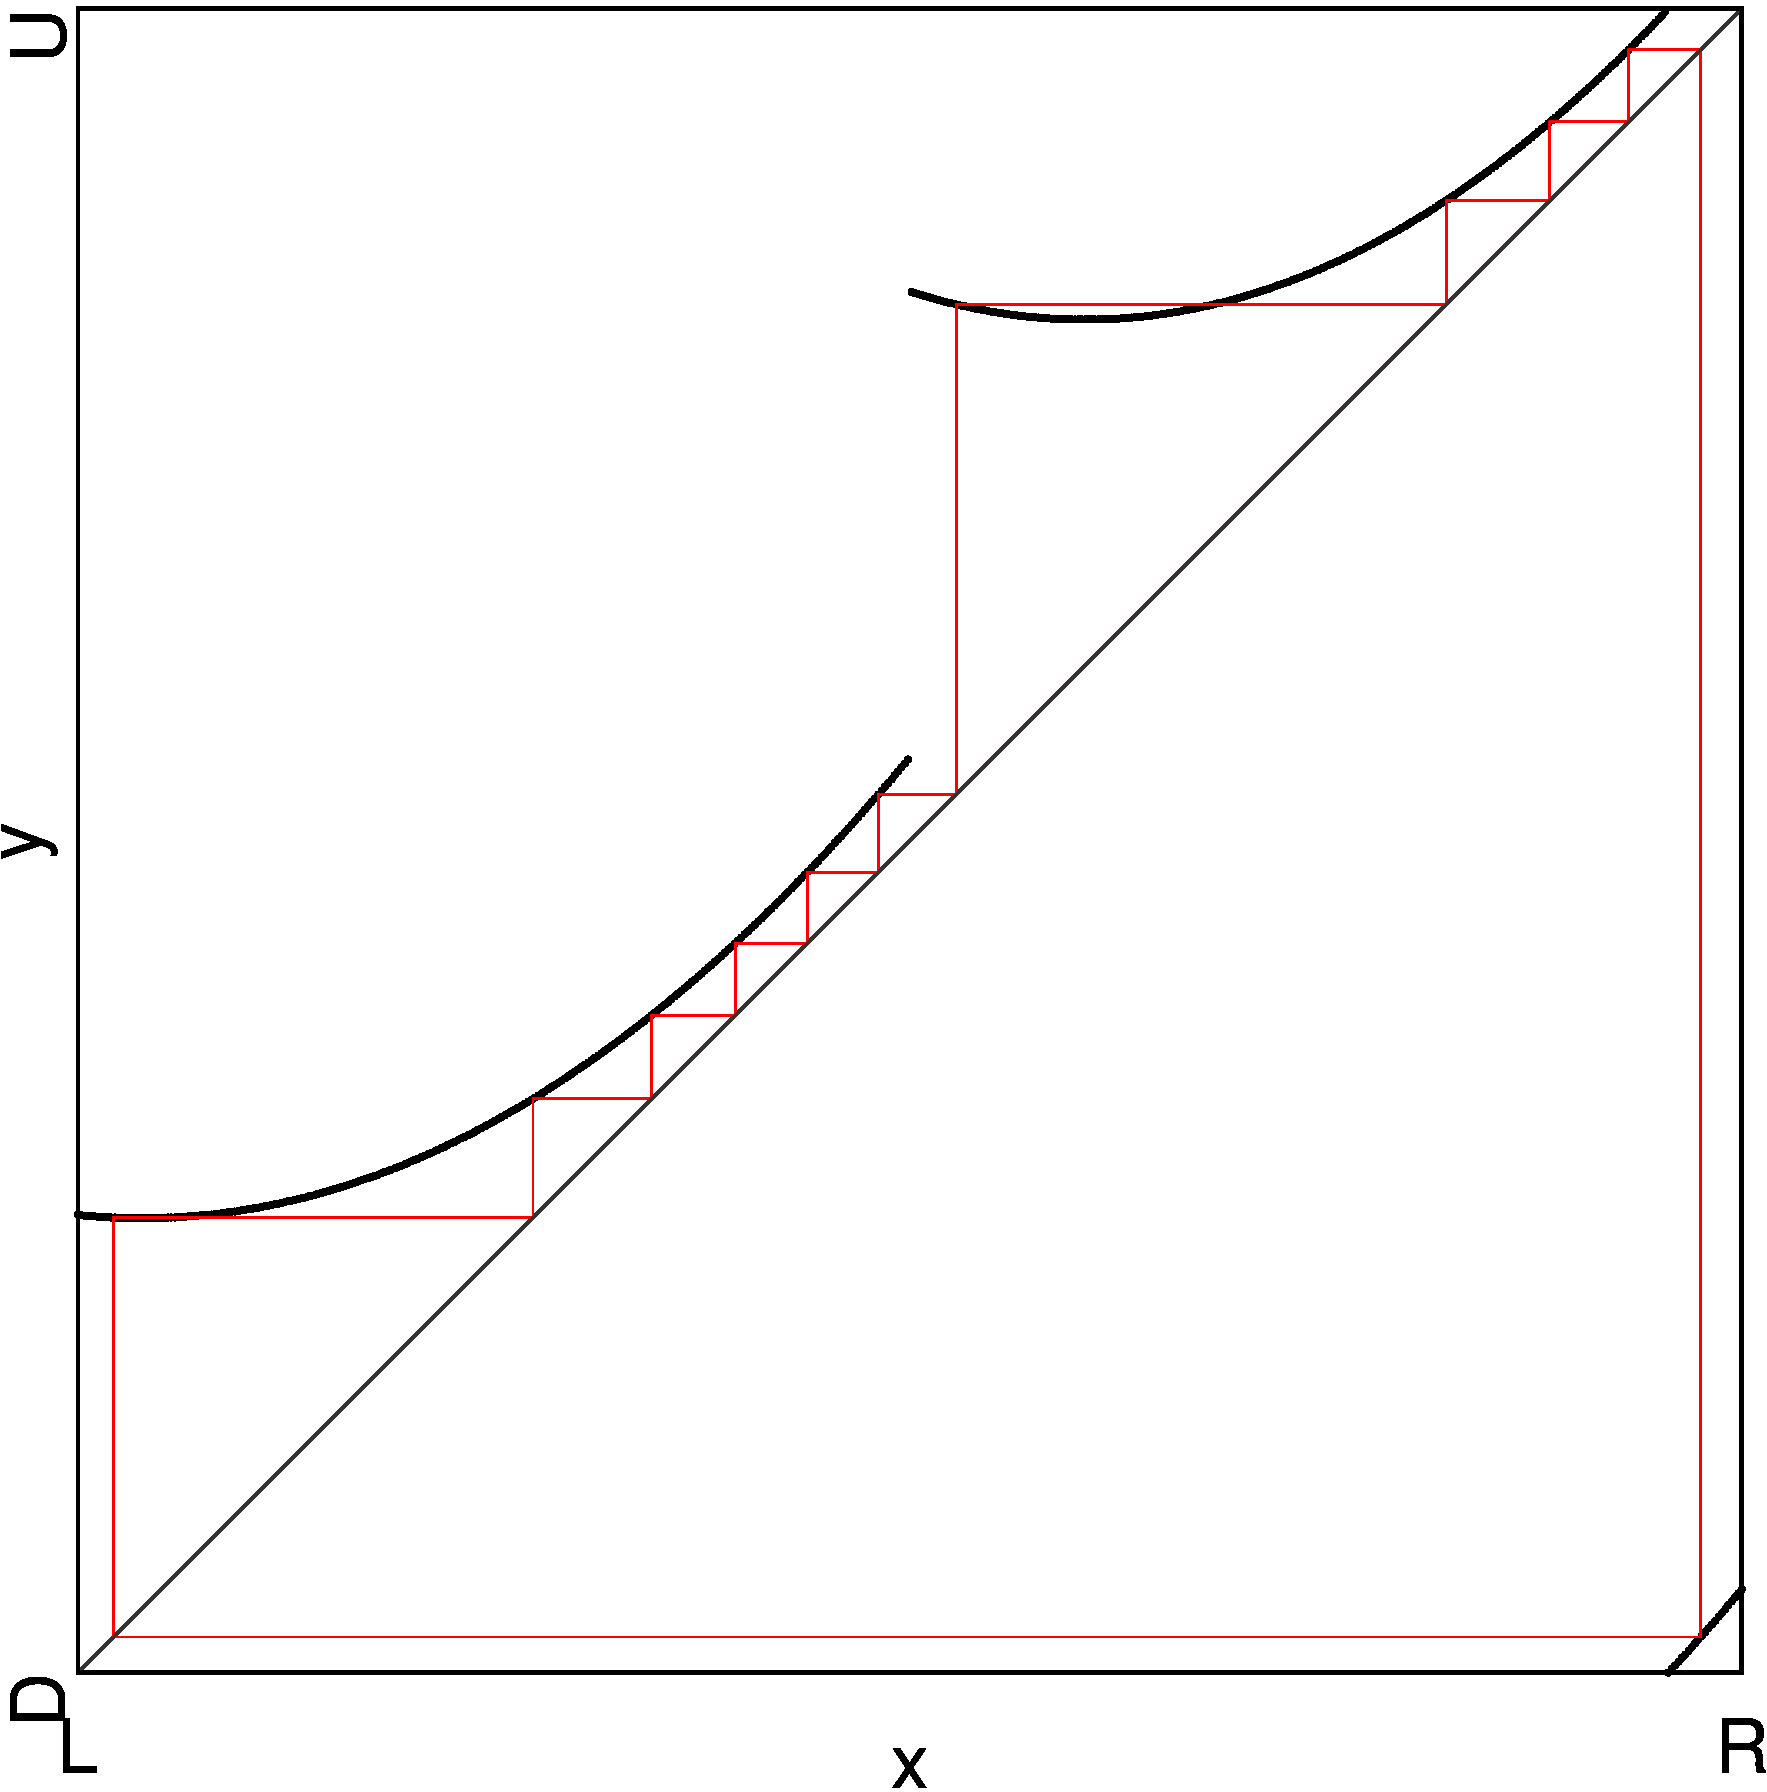
\includegraphics[height=0.7 \textheight]{60_MinimalRepr/2D_Period_Whole_noPoints/result.png}
    \end{center}
    \todo{describe type B parameter regions}
\end{frame}

\begin{frame}{The Next Step}
    Research question 3 remaining: What else can happen?

    \pause
    \vspace{2em}
    Hypothesis:
    \begin{itemize}
        \item Period Adding
    \end{itemize}
\end{frame}

\begin{frame}{Symbolic Sequences}
    Cycles are described using Symbolic Sequences.

    Sequence of Symbols indicating, on which partition of the function the points of the cycle are.

    \todo{example with graph}
\end{frame}

%\begin{frame}{What is Period Adding?}
%    \begin{columns}
%        \begin{column}{.6 \textwidth}
%            Between two parameter regions with cycles $\Cycle{L}$ and $\Cycle{R}$ there are parameter regions with:
%            \begin{itemize}
%                \item The cycle $\Cycle{LR}$ in the middle
%                \item The cycle $\Cycle{L^2R}$ between $\Cycle{L}$ and $\Cycle{LR}$
%                \item The cycle $\Cycle{LR^2}$ between $\Cycle{LR}$ and $\Cycle{R}$
%                \item etc.
%            \end{itemize}
%
%            \vspace{1em}
%            \onslide<2->{
%                The cycles are glued together \\
%                $\implies$ The periods add and so do the rotations \\
%            }
%            \onslide<3->{
%                $\implies$ Their ratio $\left(\dfrac{\text{rotations}}{\text{period}}\right)$ follows Farey-Addition
%            }
%        \end{column}
%        \begin{column}{.4 \textwidth}
%            \vspace{-3em}
%            \begin{figure}
%                \centering
%                \subfloat{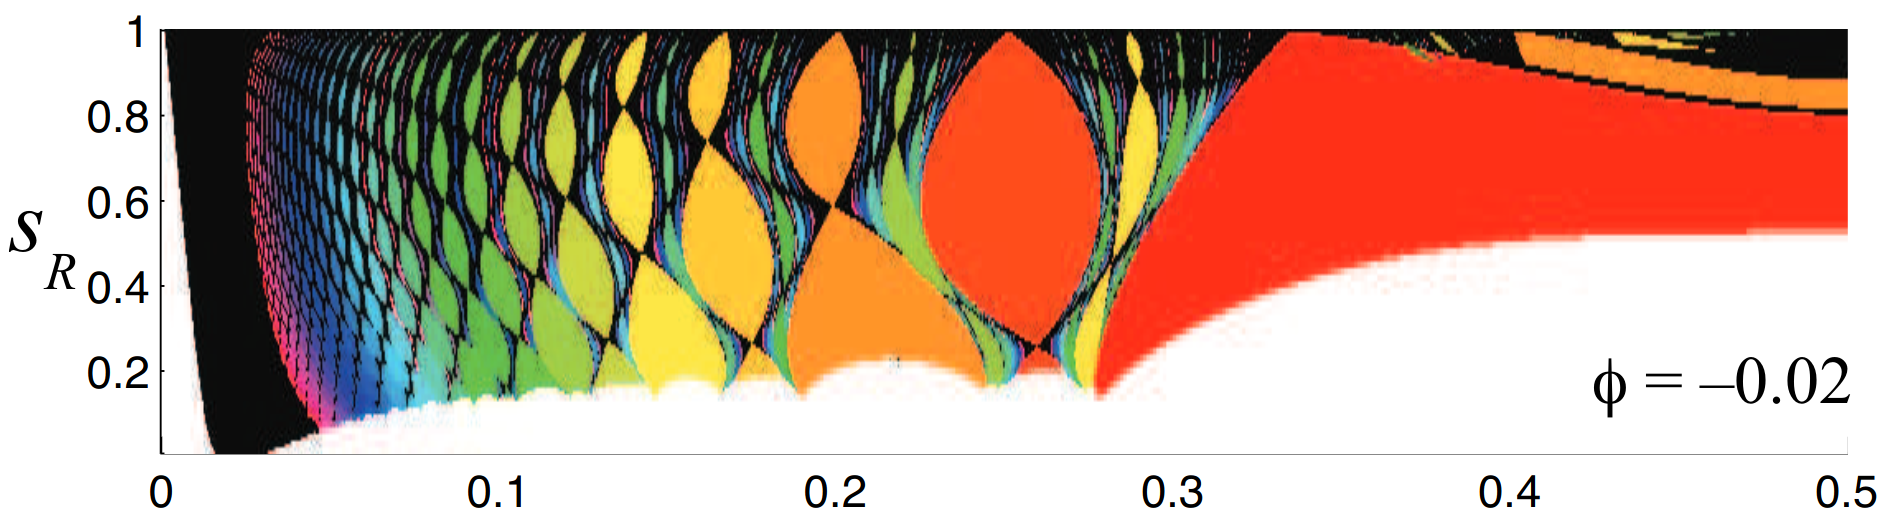
\includegraphics[width=\textwidth]{gfx/tounge_adding.png}}
%                \\
%                \subfloat{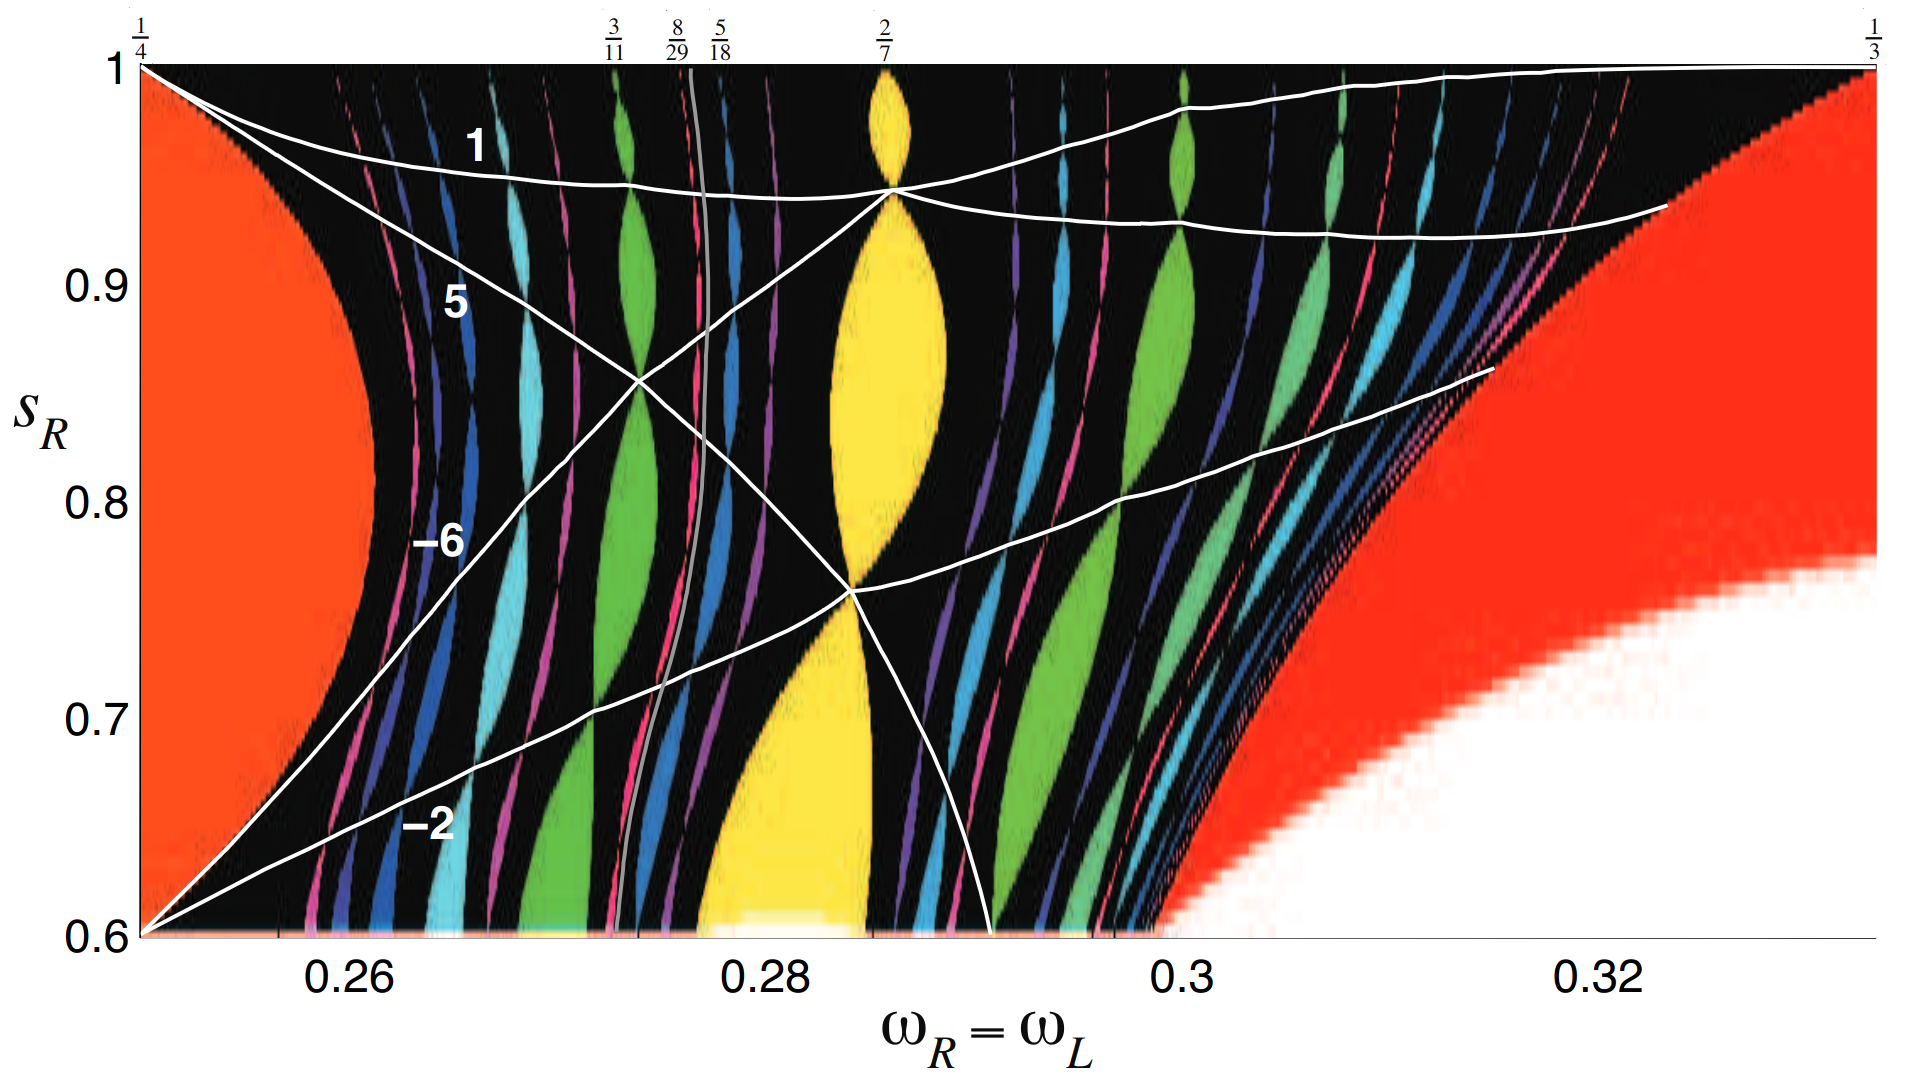
\includegraphics[width=\textwidth]{gfx/tounge_adding_zoomed.png}}
%            \end{figure}
%            \begin{flushright}
%                Pictures from \cite{simpson2010}
%            \end{flushright}
%        \end{column}
%    \end{columns}
%\end{frame}